\documentclass[10pt]{article}
\usepackage[utf8]{inputenc}
\usepackage[T1]{fontenc}
\usepackage{amsmath}
\usepackage{amsfonts}
\usepackage{amssymb}
\usepackage[version=4]{mhchem}
\usepackage{stmaryrd}
\usepackage{graphicx}
\usepackage[export]{adjustbox}
\graphicspath{ {./images/} }

\title{PHARMACOKINETICS AND METABOLISM OF VARIOUS BENZODIAZEPINES USED AS HYPNOTICS }


\author{D.D. BREIMER\\
Department of Pharmacology, Subfaculty of Pharmacy, University of Leiden,\\
Wassenaarseweg 72, 2333 Al Leiden, The Netherlands}
\date{}


\begin{document}
\maketitle


\begin{abstract}
1 In the management of insomnia with drugs, any action should be restricted to the duration of the night and residual effects should be absent during the day-time. The intermittent type of drug action desired is fundamentally different from drug treatment where a constant effect is sought.\\
2 Duration of drug action is dependent on the kinetics of distribution and elimination of the parent drug and its effective metabolites. In addition biopharmaceutical factors, such as those which promote a rapid rate of absorption, are important.\\
3 These considerations serve as a guide for a review of the kinetics and metabolism of various benzodiazepines.
\end{abstract}

\section*{Introduction}
PhARMACOKINETICS deals with the mathematical description of the processes which drugs undergo in the body, for example, absorption, distribution and elimination. Pharmacokinetic parameters, which are generally based on the relationship between plasma concentration, its time-course and the dose administered, are important for the intensity and duration of drug effects. For instance, the elimination half-life of a drug will determine its plasma concentration time-course (accumulation) during chronic administration on a fixed dosage regimen. Drug metabolism is of great interest particularly if active metabolites are formed, as is often the case with benzodiazepines. Thus, not only the pharmacokinetics of parent drug but also of its metabolites should be studied and taken into consideration.

This short review will deal with some basic requirements which a hypnotic should fulfil with respect to the duration and onset of drug action. An attempt will be made to link these requirements to pharmacokinetic principles. Finally, some pharmacokinetic data of benzodiazepines used as hypnotics and their active metabolites will be summarized.

\section*{Duration of hypnotic drug action}
Most hypnotics are prescribed for and used by nonhospitalized or ambulant patients. Therefore, the CNS-depressant effect of the drug should have declined sufficiently to be subjectively and objectively unimportant on the morning following the night of drug intake. Residual impairment of performance is undesirable, because many persons are involved in skilled activity during the day. Accordingly, the duration of drug action should in principle be limited; the pharmacokinetics of a particular hypnotic and especially its distribution and elimination behaviour are important factors in this respect (Breimer, 1977). Generally speaking, a relatively rapid rate of elimination (short elimination half-life) is an advantage for a hypnotic. However, it is also true that a long half-life of a drug does not necessarily imply a long duration of action following single dose administration.

Figure 1 shows the plasma concentration-time profile of nitrazepam after oral administration for a healthy volunteer. Absorption is rapid and after the peak concentration there is a relatively rapid decrease in the concentration, followed by a much slower decay. The more rapid phase is mainly due to drug distribution from plasma into tissues. If one assumes that the drug penetrates the brain very rapidly (in other words the brain belongs to the central compartment and thus follows the plasma concentration-time course very closely), and if one also assumes that the minimal effective concentration is above $25 \mathrm{ng} / \mathrm{ml}$, it becomes obvious that the duration of action is indeed limited to a few hours in this particular case. Obviously, a lot depends on the dose administered and the assumption that the brain concentration parallels the plasma concentration very closely. If differences in distribution exist with respect to penetration into or from the brain, a more

\begin{center}
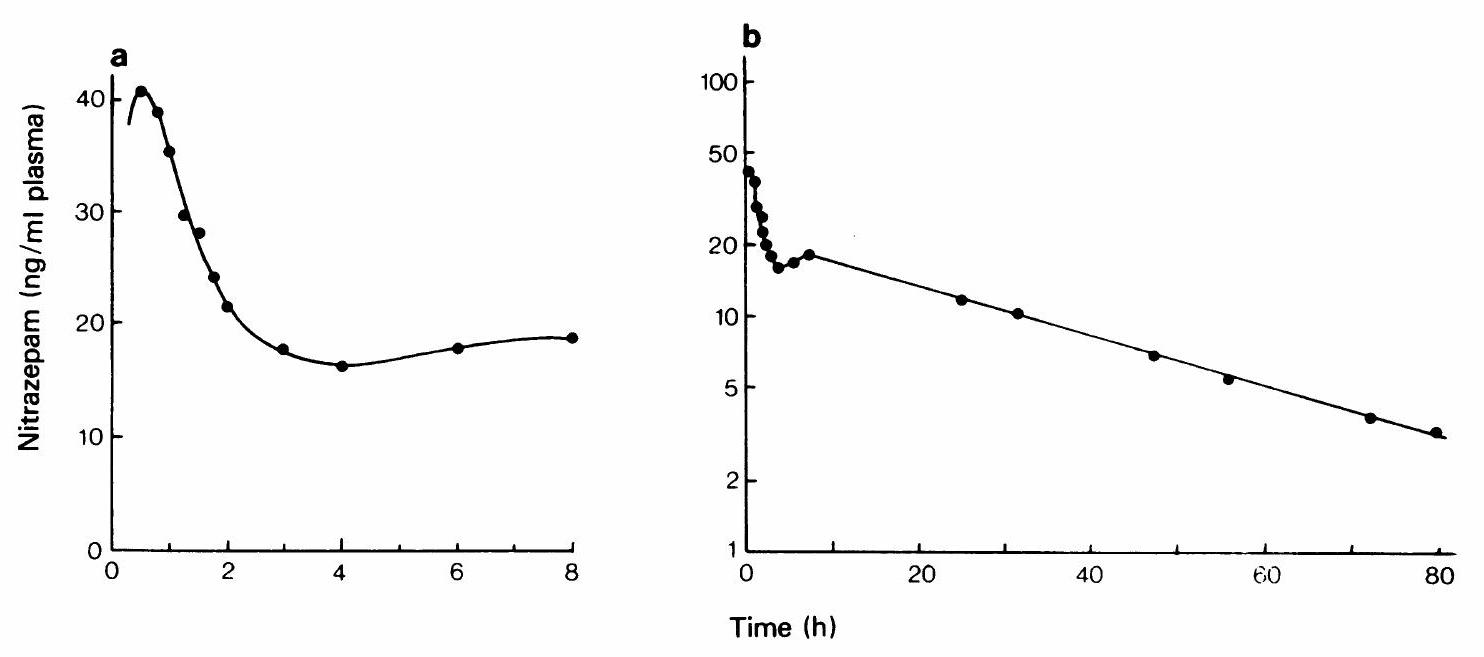
\includegraphics[max width=\textwidth]{2024_06_20_8ae6f73ba2f120e73ed4g-2}
\end{center}

Figure 1 Plasma concentration-time profile of nitrazepam following a single $5 \mathrm{mg}$ oral dose (tablet) in a healthy volunteer. The initial rapid decay is probably mainly due to distribution of the compound into tissues, whereas the dip in the curve may be due to a redistribution phenomenon caused by intercurrent intake of food (Breimer et al., 1977; courtesy of the publisher). a, Linear scale; b, log scale ( $T_{\frac{1}{2}} 28 \mathrm{~h}$ ).

complicated and less predictable situation is encountered. Therefore, in principle, two conditions should be fulfilled to obtain a short duration of hypnotic drug action despite slow elimination. Firstly, the drug has to cross the blood-brain barrier very rapidly so that there is instantaneous exchange of drug between plasma and brain. Secondly, shortly after administration the drug must become available in the blood in relatively high concentrations, otherwise the concentration profile levels out and no distinction is found between distribution and elimination phase. This initial high concentration can only be achieved if the drug is given by intravenous injection - which is not very convenient for general practice - or when very rapid absorption occurs when the drug is given orally. Thus, an initial high concentration may be obtained, as is shown for nitrazepam in Figure 1. If brain concentrations closely follow plasma concentrations of this hypnotic, it might be short acting at low doses, despite its slow terminal elimination phase. But an important further question is: What happens if a hypnotic is taken every evening, because many patients tend to take a hypnotic in this way? In hypnotic drug therapy one is in fact pursuing an intermittent type of drug action when the drug is given repeatedly. This type of drug therapy is fundamentally different from most others, because in this case a constant effect at every time of day and night is generally desirable (for example, anticonvulsants, digoxin). In such a case the plasma concentration should be as constant as possible and consistently well above the minimal effective concentration. But for hypnotics such a situation is in fact undesirable unless one is also interested in day-time sedation as may sometimes be the case.

Figure 2 shows theoretical plasma level profiles of two hypnotics with different half-lives, when they are given every 24 hours. If the compound with a halflife of $6 \mathrm{~h}$ is given in this way, no accumulation occurs and one is indeed dealing with an intermittent type of drug action. If, on the other hand, the elimination half-life of the drug is $24 \mathrm{~h}$ or longer, then it will accumulate after chronic administration. Such a situation is, for instance, encountered for butobarbitone with a half-life of $40 \mathrm{~h}$ (Breimer, 1976). Accumulation represents an undesirable situation, although one might argue that the patient will probably not be asleep all day despite the relatively high drug concentration. This indicates that adaption or tolerance to the effect of the drug develops, which may ultimately lead to drug dependence. This is a very undesirable situation but a condition well known in chronic barbiturate users. If one seeks to restrict the treatment to night-time sedation and if one also wants to give the drug every night, then a short elimination half-life is certainly a great advantage. Unfortunately, few hypnotics fulfil that requirement.

\section*{Onset of hypnotic drug action}
Hypnotics are most frequently prescribed for patients who experience difficulty in getting to sleep. They require a pharmaceutical formulation (dosage

\begin{center}
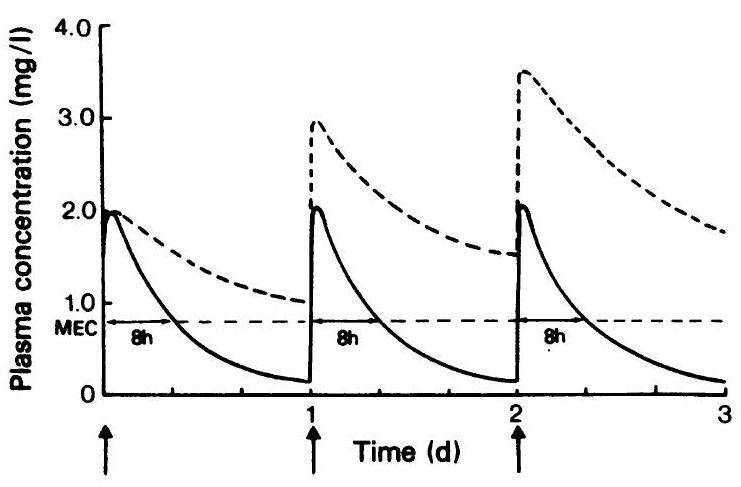
\includegraphics[max width=\textwidth]{2024_06_20_8ae6f73ba2f120e73ed4g-3}
\end{center}

Figure 2 Theoretical plasma concentration profile of two hypnotics with different elimination half-lives: solid line, $6 \mathrm{~h}$; dotted line, $24 \mathrm{~h}$, during nightly administration. It demonstrates that real intermittent therapy can only be achieved with a rapidly eliminated drug, whereas accumulation will occur with hypnotics that are slowly eliminated. MEC refers to the minimal effective concentration; in hypnotic therapy the drug effect should last $8 \mathrm{~h}$ or less (Breimer, 1976; courtesy of the publisher). $D=100 \mathrm{mg} ; \Delta t=24 \mathrm{~h} ; V d=50$.

form) from which the active compound is rapidly absorbed. If this does not happen, early sleep may not be obtained and the patient is tempted to take a second dose, which may lead to overdosing and prolonged effect. Biopharmaceutical factors governing the rate and extent of absorption are very important in this respect, where a rapid rate of absorption is particularly desirable (Breimer, 1976). The principle of rapid absorption is very important, not only with respect to the onset of action but also with regard to the duration of action. It was mentioned before that with a drug having a long elimination half-life, a short duration of action can be obtained, provided that a relatively high concentration is initially available; the only way of reaching that high concentration orally is by rapid absorption.

Differences in rates of absorption may account for discrepancies in drug effects: for instance, Kales' group recently published a paper on flunitrazepam efficiency as a hypnotic (Bixler et al., 1977). The 2$\mathrm{mg}$ dose was effective but the $1 \mathrm{mg}$ was not. This contrasts with an earlier study which showed that $1 \mathrm{mg}$ and even $0.25 \mathrm{mg}$ was effective (Kales \& Scharf, 1973). The discrepancy may very well be due to differences in rates of absorption of the drug formulations used. This is an often neglected aspect of hypnotic therapy, but it does have major consequences: with rapid absorption one may achieve a rapid onset of action with a relatively low dose and thereby also limit the duration of action.

\section*{Pharmacokinetics and metabolism of benzodiazepines}
The pharmacokinetics of some benzodiazepines, particularly those regularly used as hypnotics, will be reviewed briefly against the background of the above points.

In Table 1 the elimination half-lives of various

Table 1 Elimination half-lives of benzodiazepines and active metabolites in healthy adults

\begin{center}
\begin{tabular}{|c|c|c|c|c|}
\hline
Generic name & \begin{tabular}{l}
Half-life of \\
parent drug \\
(h) \\
\end{tabular} & Active metabolite & \begin{tabular}{l}
Half-life of \\
metabolite \\
(h) \\
\end{tabular} & References \\
\hline
Nitrazepam & $18-13$ & Probably none &  & \begin{tabular}{l}
(Breimer et al., 1977; De Boer \\
et al., 1978) \\
\end{tabular} \\
\hline
\begin{tabular}{l}
Flurazepam \\
Flunitrazepam \\
\end{tabular} & \begin{tabular}{l}
Very short \\
$15-30$ \\
\end{tabular} & \begin{tabular}{l}
N-desalkylflurazepam \\
7-Amino-derivative \\
\end{tabular} & \begin{tabular}{l}
$24-48$ \\
$23 \pm 4$ \\
\end{tabular} & \begin{tabular}{l}
(Kaplan et al., 1973) \\
(Cano et al., 1977; Amrein \\
et al., 1976; Wendt, 1976) \\
\end{tabular} \\
\hline
Diazepam & $14-90$ & \begin{tabular}{l}
Desmethyl-derivative \\
Desmethyl-derivative \\
3-Hydroxy-derivative \\
(temazepam) \\
\end{tabular} & \begin{tabular}{c}
$31 \pm 8$ \\
$30-60$ \\
$4-10$ \\
\end{tabular} & \begin{tabular}{l}
(Mandelli et al., 1978) \\
(Fucella et al., 1977) \\
\end{tabular} \\
\hline
\begin{tabular}{l}
Temazepam \\
Oxazepam \\
Triazolam \\
Chlordiazepoxide \\
\end{tabular} & \begin{tabular}{l}
$4-10$ \\
$6-24$ \\
$5-10$ \\
$7-14$ \\
\end{tabular} & \begin{tabular}{l}
Oxazepam \\
Probably none \\
Probably none \\
7-a-Hydroxy-triazolam \\
Desmethyl-derivative \\
Demoxepam \\
Desmethyldiazepam \\
\end{tabular} & $6-24$ & \begin{tabular}{l}
(Sjoqvist \& Sundwall, 1977) \\
(Fucella et al., 1977) \\
(Sjoqvist \& Sundwall, 1977) \\
(Eberts et al., 1979) \\
(Boxenbaum et al., 1977) \\
\end{tabular} \\
\hline
\begin{tabular}{l}
Lorazepam \\
Clorazepate \\
\end{tabular} & $9-22$ & \begin{tabular}{l}
Probably none \\
Desmethyldiazepam \\
\end{tabular} & $30-60$ & \begin{tabular}{l}
(Greenblatt et al., 1977) \\
(Post et al., 1977) \\
\end{tabular} \\
\hline
\end{tabular}
\end{center}

benzodiazepines are given, including those of a number of active metabolites. An important aspect in discussing benzodiazepines is the formation of active metabolites. If one considers the pharmacokinetics of benzodiazepines in relation to their therapeutic effect, the concentrations and concentration timecourse of the active metabolites must also be taken into account. The metabolites of diazepam are the most well-known and extensively studied, and some have been marketed as separate drugs.

The data in Table 1 underline the variation in the elimination half-lives of benzodiazepines. As mentioned before, a long half-life does not necessarily imply a long duration of action after single dose administration, but it does mean accumulation if the dosage interval is short relative to its half-life.

\section*{Nitrazepam}
Recently, very sensitive and specific methods were developed for the determination of nitrazepam in plasma, using gas chromatography with electron capture detection (Kangas, 1977; De Boer et al., 1978). An example of the plasma concentration time-course of nitrazepam following a single dose is shown in Figure 1. Absorption is quite rapid, and the initial rapid decrease is caused mainly by distribution of the drug from plasma into tissues, whereas elimination is rather slow with an average elimination half-life of $28 \mathrm{~h}$ (de Boer et al., 1978) or $30 \mathrm{~h}$ (Breimer et al., 1977). Similar half-lives were published by Rieder (1973) and Kangas et al. (1977). The sudden rise and fall in the curve of Figure 1 is probably due to a redistribution phenomenon caused by the intercurrent intake of food (Breimer et al., 1977), an observation similar to that made for diazepam (Kortilla \& Kangas, 1977).

The situation during chronic administration of nitrazepam every night is simulated in Figure 3. There will be a certain degree of accumulation particularly if the half-life is long relative to the dosage interval. We measured the nitrazepam concentration in nine hospitalized patients at 09.00 in the morning, after they had been given nitrazepam $5 \mathrm{mg}$ for several previous nights. There was considerable interindividual variation in the measured concentration, with an average value of $72 \mathrm{ng} / \mathrm{ml}$. In single dose studies the concentrations about $10 \mathrm{~h}$ following drug administration are generally below $20-30 \mathrm{ng} / \mathrm{ml}$. In elderly or geriatric patients in particular, the risk of accumulation is substantial because they have a significantly longer elimination half-life than younger people (Kangas et al., 1979).

Nitrazepam is metabolized in man in part by the successive enzymic bio-transformation steps of nitro-

\begin{center}
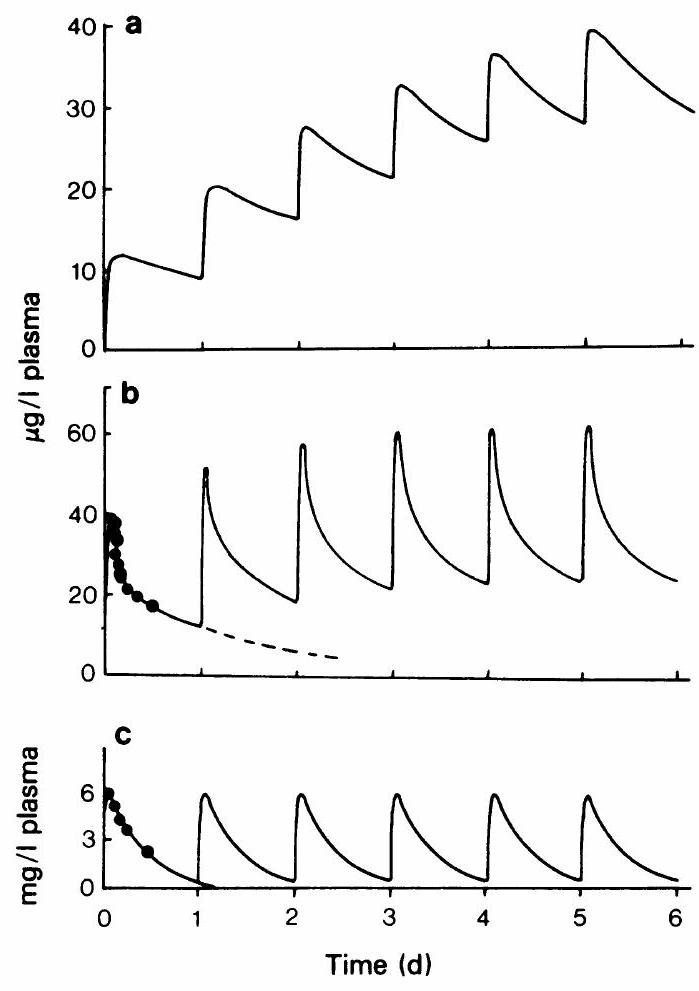
\includegraphics[max width=\textwidth]{2024_06_20_8ae6f73ba2f120e73ed4g-4}
\end{center}

Figure 3 Plasma concentration profile of three hypnotic benzodiazepines during nightly administration. a, N-desalkylflurazepam; b, nitrazepam $5 \mathrm{mg}$; c, temazepam $20 \mathrm{mg}$. Calculation of the curves is based on the experimental concentrations obtained after a single oral dose and assuming an elimination half-life of $7 \mathrm{~h}$ for temazepam, $24 \mathrm{~h}$ for nitrazepam and $3 \mathrm{~d}$ for $\mathrm{N}$-desalkylflurazepam. The latter compound is an active metabolite of flurazepam and the concentration profile simulates the situation of nightly administration of flurazepam $30 \mathrm{mg}$.

reduction to the aromatic amine followed by acetylation to the acetamido compound (Beyer \& Sadee, 1969). This acetylation step is controlled by the same genetic polymorphism as sulphadimidine (Karim \& Price Evans, 1976). These metabolites do not possess hypnotic activity.

\section*{Flurazepam}
Kaplan et al. (1973) have studied the kinetics of flurazepam and its metabolites (hydroxyethyl derivative and the $\mathrm{N}$-1-desalkyl derivative) at doses of $30 \mathrm{mg}$ daily. Only trace amounts of unchanged drugs were measured, whereas the hydroxyethyl\\
metabolite was measurable for several hours after each dose. Accumulation of this metabolite was not observed. The major metabolite was the N-1-desalkyl derivative, which was shown to have an elimination half-life ranging from $47-100 \mathrm{~h}$ in the four healthy volunteers. Peak concentrations after a single dose were 10 to $22 \mathrm{ng} / \mathrm{ml}$ blood and increased after 2 weeks of treatment ( $30 \mathrm{mg}$ every night) to 49 $142 \mathrm{ng} / \mathrm{ml}$. Thus, significant accumulation of this metabolite occurs during continuous administration of flurazepam. In Figure 3 this situation has been simulated.

As this desalkylated metabolite of flurazepam has psychopharmacological activity similar to that found for flurazepam in animal studies (Randall \& Kappell, 1973), it might contribute to the hypnotic and persistent sedative action of flurazepam. Kales et al. (1976) have discussed the accumulation of active metabolites in relation to the effectiveness of flurazepam as evaluated in sleep laboratory studies, where the drug did not reach peak effectiveness until the second and third consecutive drug nights. One might need a relatively high concentration of this metabolite to obtain optimal hypnotic effect, but one should realize at the same time that relatively high concentrations of this active compound will be present in the body during the day as well.

\section*{Diazepam}
Despite its major use as a minor tranquillizer, diazepam has been included in this brief review, because of evidence that single doses of diazepam can be used very effectively for sleep induction (Nicholson \& Stone, 1977). There are three major metabolites of diazepam with anti-anxiety activity They have been marketed as single drugs (3hydroxydiazepam or temazepam, and oxazepam) or as a pro-drug (N-desmethyldiazepam as clorazepate). Temazepam and oxazepam will be dealt with separately

Numerous investigations have been published on the pharmacokinetics and metabolism of diazepam, so that no attempt will be made to refer to all the available literature (for review, see Mandelli et al., 1978). The elimination half-life of diazepam varies from $14-90 \mathrm{~h}$, whereas generally in an individual subject the half-life of desmethyldiazepam is slightly longer. The half-life of diazepam increases with age. On chronic administration of diazepam (for instance, three times daily) accumulation to relatively high steady-state levels will occur for diazepam and desmethyldiazepam (Eatman et al., 1977).

If the parent drug is given to patients to obtain a continuous anti-anxiety effect, this constant level may represent a desirable situation. When used only as a sleep-inducing agent, diazepam should not be given every night

\section*{Temazepam (3-hydroxydiazepam)}
Recently temazepam has been shown to be an effective sleep-inducing agent (Nicholson \& Stone, 1976). It has a short-life of $5-8 \mathrm{~h}$ (Fuccella et al., 1977) and no active metabolites are formed, except oxazepam to a very minor extent. After seven consecutive night-time administrations of temazepam to healthy volunteers, no changes in halflife became apparent and plasma concentrations on the seventh were similar to those on the first day (Fuccella et al., 1977). In Figure 3 the situation of repetitive drug administration (every night) has been simulated. Thus, from the pharmacokinetic point of view, temazepam seems to be a suitable hypnotic for administration every night.

\section*{Oxazepam}
Oxazepam is predominantly used as an anti-anxiety agent and its pharmacokinetics have recently been reviewed (Sjoqvist $\&$ Sundwall, 1977). It has a mean elimination half-life of $10-12 \mathrm{~h}$ and is mainly bioinactivated through glucuronidation. Although these pharmacokinetic properties are appropriate to its use as a hypnotic, its effectiveness has not been proved adequately. It is possible that its relatively polar properties prevent rapid absorption and rapid brain penetration.

\section*{Triazolam}
Triazolam is a benzodiazepine derivative with a triazole structure attached at the 3,4-position to the azepine ring. Several clinical studies have shown it to be an effective hypnotic. Preliminary data on the pharmacokinetics and metabolism of triazolam indicate that the elimination half-life is quite short (mean of about $5 \mathrm{~h}$; Eberts et al., 1979). Multiple dose studies (every night for $7 \mathrm{~d}$ ) agree that there is no appreciable accumulation of parent compound nor metabolites. One of the major metabolites ( $\alpha$ hydroxytriazolam) seems to have $50-100 \%$ of the pharmacological activity of the parent compound and is probably also rapidly eliminated (Eberts et al., 1979). More definite data on the pharmacokinetics and metabolism of triazolam are required, but so far, at least from the pharmacokinetic point of view, it seems a promising hypnotic.

\section*{Flunitrazepam}
Flunitrazepam is a fluorinated and $\mathrm{N}$-methylated analogue of nitrazepam, which is used as an intravenous anaesthetic agent and also as a hypnotic. Its oral plasma concentration-time profile is similar to that of nitrazepam (Figure 1) and its elimination\\
half-life varies from 15-30 h (Cano et al., 1977; Amrein et al., 1976). On single dose administration, the intensity of the sedative effect of the drug correlated with the plasma concentrations during the distribution phase; in normal dose ( $2 \mathrm{mg}$ ) the effect disappeared before the elimination phase was reached (Amrein, 1978). Data on the pharmacokinetics of flunitrazepam during repetitive administrations are not available.

With respect to the metabolism of flunitrazepam in man, as for nitrazepam, the nitro group is reduced to the derivative and $\mathrm{N}$-demethylation also occurs, which in both cases leads to the formation of active metabolites (Wendt, 1976). The elimination half-lives of these compounds are relatively long (Table 1), which may lead to accumulation on chronic administration.

\section*{References}
AMREIN, R. (1979). Clinical and psychometric effects of flunitrazepam observed during the day in relation to pharmacokinetic data. In Proceedings Northern European Symposium on Sleep Research. Basel, September 25-27 (in press).

AMREIN, R., CANO, J.P. \& HƯGIN, W. (1976). Pharmakokinetische und pharmakodynamische Befunde nach einmaliger intravenoser, intramuskularer und oraler Applikation von "Rohypnol". In Bisherige Erfahrungen mit "Rohypnol" (Flunitrazepam) in der Anasthesiologie und Intensivtherapie. Ed. Hügin, W., Hossli, G \& Gemperle, M. Pp. 39-56. Basel: Roche Editiones.

BEYER, K.H. VON \& SADEE, W. (1969). Spektrophotometrische Bestimmung von 5-phenyl-1,4-benzodiazepine Derivaten und Untersuchungen uber den Metabolismus des Nitrazepam. Arzneimittel-Forsch., 19, 1929-1931.

BIXLER, E.O., KALES, A., SOLDATOS, C.R. \& KALES, J.D. (1977). Flunitrazepam, an investigational hypnotic drug; sleep laboratory evaluations. J. clin. Pharmac., 17, 569-578.

BOXENBAUM, H.G., GEITNER, K.A., JACK, M.L., DIXON, W.R., SPIEGEL, H.E., S/MINGTON, J. CHRISTIAN, R., MOORE, J.D., WEISSMAN, L. \& KAPLAN, S.A. (1977). Pharmacokinetic and biopharmaceutical profiles of chlordiazepoxide $\mathrm{HCl}$ in healthy subjects: single dose studies by the intravenous, intramuscular and oral routes. J. Pharmacokin. Biopharm., 5, 3-24.

BREIMER, D.D. (1976). Pharmacokinetic and biopharmaceutical aspects of hypnotic drug therapy. In Clinical Pharmacy and Clinical Pharmacology. Ed. Gouveia, W.A., Tognoni, G. \& Van der Klein, E. Pp. 19-42. Amsterdam: Elsevier/North-Holland Biomedical.

BREIMER, D.D. (1976). Pharmacokinetics of butobarbital after single and multiple oral doses in man. Eur. J. clin. Pharmac., 10, 263-271.

BREIMER, D.D. (1977). Clinical pharmacokinetics of hypnotics. Clin. Pharmacokin., 2, 93-109.

BREIMER, D.D., BRACHT, H. \& DE BOER, A.G. (1977). Plasma level profile of nitrazepam following oral administration. Br. J. clin. Pharmac., 4, 709-711.

\section*{Conclusions}
The pharmacokinetics of parent drug and active metabolites of benzodiazepines should be carefully considered when they are used as hypnotics. Their elimination half-life is an important variable to judge whether substantial accumulation will occur on nightly administration. Those with a relatively short half-life are preferable as they will allow the real intermittent type of drug action desired in hypnotic therapy. In addition, attention should be paid to biopharmaceutical factors of hypnotic drug formulations and especially to those favouring a rapid rate of absorption. Thus, not only is a rapid onset of drug action achieveable, but also the duration of drug action may be limited because a relatively low dose will be effective.

CANO, J.P., SOLIVA, M., HARTMANN, D., ZIEGLER, W.H. \& AMREIN, R. (1977). Bioavailability of various galenic formulations of flunitrazepam. Arzneimittel-Forsch., 27, 2383-2395.

DE BOER, A.G., ROST-KAISER, J. BRACHT, H. \& BREIMER, D.D. (1978). Assay of underivatized nitrazepam and clonazepam in plasma by capillary gas chromatography applied to pharmacokinetic and bioavailability studies in humans. J. Chromatogr. - Biomed. Appl., 145, 105-114.

EATMAN, F.B., COLBURN, W.A., BOXENBAUM, H.G., POSMANTER, H.N., WEINFELD, R.E., RONFELD, R., WEISSMAN, L., MOORE, J.D., GIBALDI, M. \& KAPLAN, S.A. (1977). Pharmacokinetics of diazepam following multiple dose oral administration to healthy human subjects. J. Pharmacokin. Biopharm., 5, 481-494.

EBERTS, F.S., KO, H. \& THOMAS, R.C. (1979). Metabolism and pharmacokinetics of triazolam (in preparation)

FUCELLA, L.M., BOLCIONI, G., TAMASSIA, V., FERRARIO, L. \& TOGNONI, G. (1977). Human pharmacokinetics and bioavailability of temazepam administered in soft gelatin capsules. Eur. J. clin. Pharmac., 12, 383-386.

GREENBLATT, D.J., JOYCE, T.H., COMER, W.H., KNOWLES, J.A., SHADER, R.I., KYRIAKOPOULOS, A.A., MACLAUGHLIN, D.S. AND RUELIUS, H.W. (1977). Clinical pharmacokinetics of lorazepam. II. Intramuscular injection. Clin. Pharmac. Ther., 21, 222-230.

KALES, A., BIXLER, E.O., SCHARF, M. \& KALES, J.D. (1976). Sleep laboratory studies of flurazepam: a model evaluating hypnotic drugs. Clin. Pharmac. Ther., 19, 576-583.

KALES, A. \& SCHARF, M.D. (1973). Sleep laboratory and clinical studies of the effects of benzodiazepines on sleep: flurazepam, diazepam, chlordiazepoxide and RO 5-4200. In The Benzodiazepines. Ed. Garrattini, S., Mussini, E. \& Randall, L.O. Pp. 577-598. New York: Raven.

KANGAS, L. (1977). Comparison of two gas-liquid chromatographic methods for the determination of nitrazepam in plasma. J. Chromatogr., 136, 259-270.

KANGAS, L., KANTO, J. \& SYVALAHTI, E. (1977). Plasma nitrazepam concentration after an acute intake and their correlation to sedation and serum growth hormone levels. Acta Pharmac. Toxic., 41, 65-73.

KANGAS, L., LISALO, E., KANTO, J., LEHTINEN, V., PYNNONEN, S., RUIKKA, I., SALMINEN, J., SILLANPAA, M. \& SYVALAHTI, E. (1979). Human pharmacokinetics of nitrazepam: effect of age and diseases. Eur. J. clin. Pharmac. (in press).

KAPLAN, S.A., DE SILVA, J.A.F., JACK, M.L., ALEXANDER, K. STROJNY, N., WEINFELD, R.E., PUGLIST, C.V. \& WEISSMAN, L. (1973). Blood level profile in man following chronic oral administration of flurazepam hydrochloride. J. pharm. Sci., 62, 1932-1935.

KARIN, A.K.M.B. \& PRICE EVANS, D.A. (1976). Polymorphic acetylation of nitrazepam. J. med. Genet., 13, 17-19.

KLOTZ, U., AVANT, G.R., HAYUMPA, A., SCHENKER, S. \& WILKINSON, G.R. (1975). The effects of age and liver disease on the disposition and elimination of diazepam in adult man. J. clin. Invest., 55, 347-359.

KORTILLA, K. \& KANGAS, L. (1977). Unchanged protein binding and the increase of serum diazepam levels after food intake. Acta Pharmac. Toxic., 40, 241-246.

MANDELLI, M., TOGNONI, G. \& GARATTINI, S. (1978). Clinical pharmacokinetics of diazepam. Clin. Pharmacokin., 3, 72-91.\\
NICHOLSON, A.N. \& STONE, B.M. (1977). Effectiveness of diazepam and its metabolite, 3-hydroxydiazepam (temazepam), for sleep during the day. J. Physiol., Lond., 270, 29P.

NICHOLSON, A.N. \& STONE, B.M. (1976). Effect of metabolite of diazepam, 3-hydroxydiazepam (temazepam), on sleep in man. Br. J. clin. Pharmac., 3, 543-550.

POST, C., LINDGREN, S., BERTLER, A. \& MALMGREN, H. (1977). Pharmacokinetics of N-desmethyldiazepam in healthy volunteers after single daily doses of dipotassium clorazepate. Psychopharmacology, 53, 105-109.

RANDALL, L.O. \& KAPPELL, B. (1973). Pharmacological activity of some benzodiazepines and their metabolites. In The Benzodiazepines. Ed. Garrattini, S. Mussini, E. \& Randall, L.O. Pp. 27-51. New York: Raven.

RIEDER, J. (1973). Plasma levels and derived pharmacokinetic characteristics of unchanged nitrazepam in man. Arzneimittel-Forsch., 23, 212-218.

SJOQVIST, F. \& SUNDWALL, A. (ed.) (1977). The pharmacokinetic profile of oxazepam. Acta Pharmac. Toxic., 40, suppl. 1 .

WENDT, G. (1976). Schicksal des Hypnotikum Flunitrazepam im menschlichen Organismus. In Bisherige Erfahrungen mit "Rohypnol" (Flunitrazepam) in der Anasthesiologie und Intensivtherapie. Ed. Hügin, W., Hossli, G. \& Gemperle, M. Pp. 27-38. Basel: Roche Editiones.


\end{document}